% Compile from the repository root, or adapt the paths below.
% Required packages: graphicx, amsmath, amssymb.

\begin{figure*}[t]
  \centering
  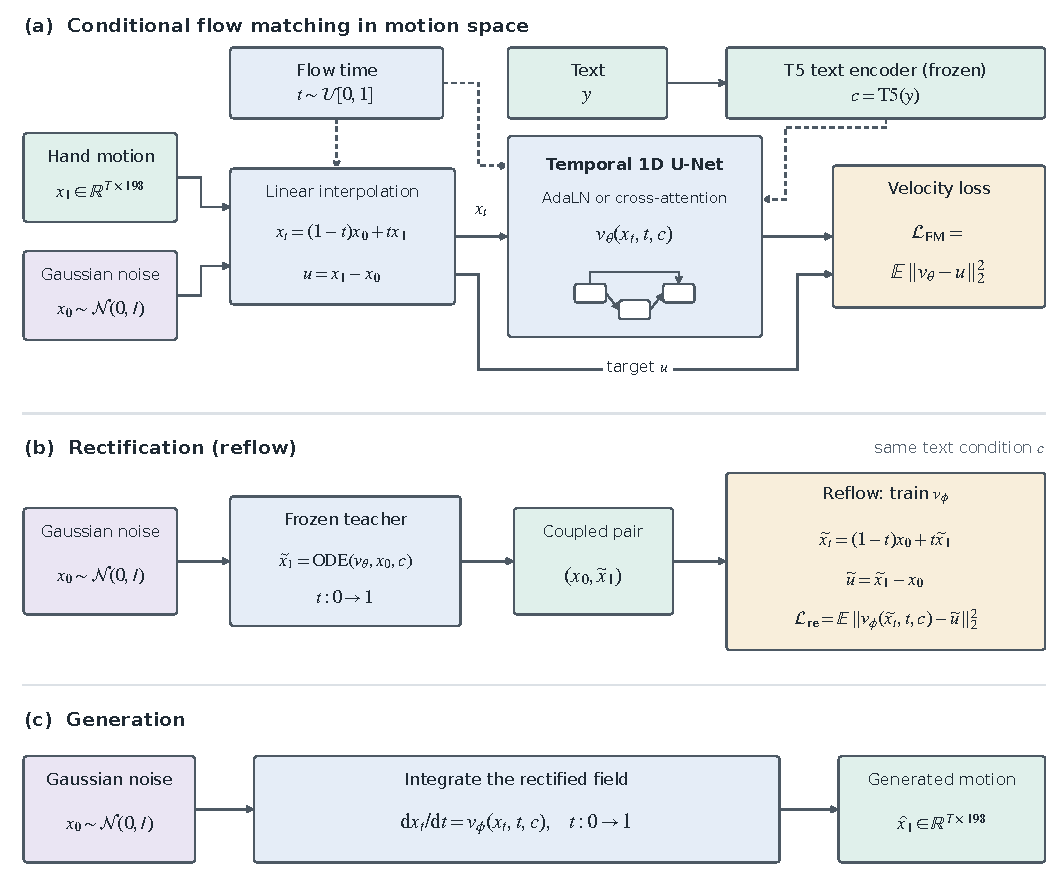
\includegraphics[width=\textwidth]{materials/figures/hand_flow_base/rectified_flow_matching.pdf}
  \caption{Proposed rectified-flow pipeline for text-conditioned bimanual hand
  motion generation.
  (a) A temporal 1D U-Net learns the velocity from Gaussian noise $x_0$ to motion
  $x_1$ along linear interpolation paths, using the target $u=x_1-x_0$.
  The text condition is $c=\mathrm{T5}(y)$, with a frozen text encoder;
  AdaLN and textual cross-attention denote alternative U-Net conditioning designs.
  (b) A frozen teacher generates $\widetilde{x}_1$ from $x_0$ under the same
  condition. Reflow trains $v_\phi$ on straight paths between these coupled
  endpoints, preserving the noise that generated each synthetic motion.
  (c) Integrating the rectified field from $t=0$ to $t=1$ generates a motion
  sequence. Dashed arrows denote conditioning.}
  \label{fig:rectified-flow-pipeline}
\end{figure*}

\begin{figure*}[t]
  \centering
  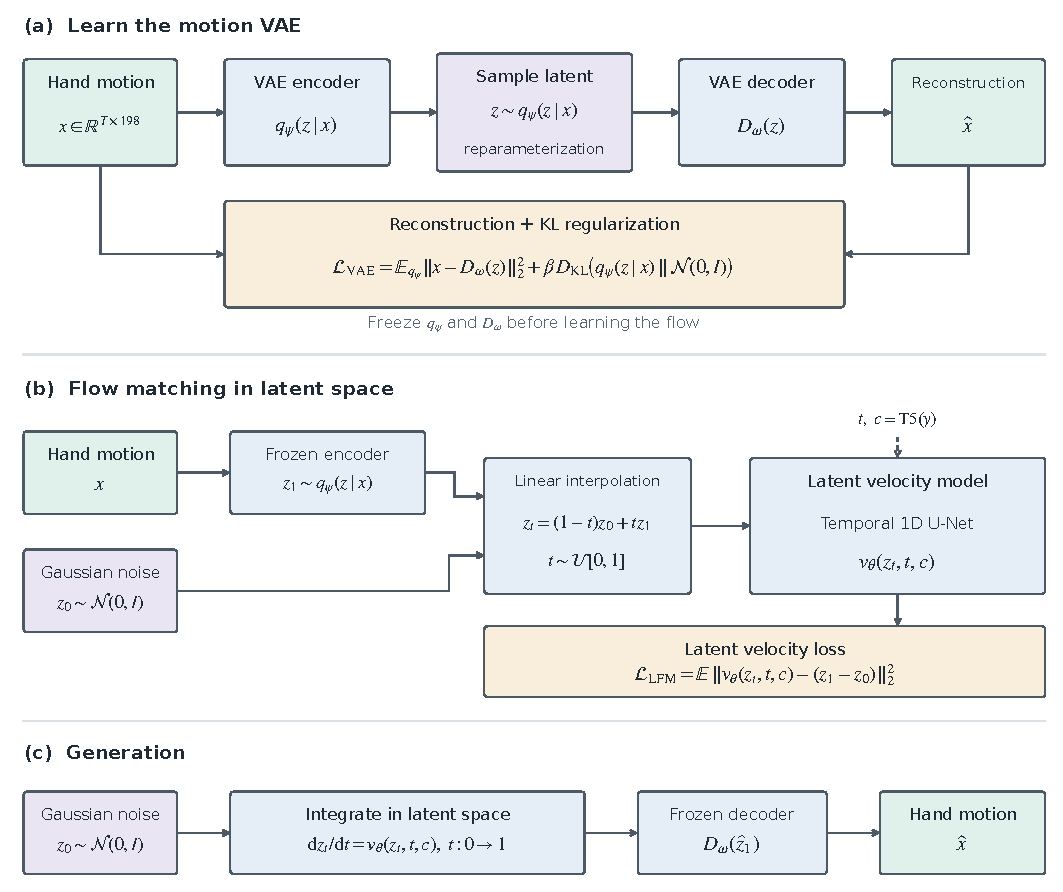
\includegraphics[width=\textwidth]{materials/figures/latent_hand_flow/latent_flow_matching.pdf}
  \caption{Proposed VAE latent-flow pipeline for text-conditioned bimanual
  hand motion generation.
  (a) The motion VAE is trained with a reconstruction loss and a weighted KL
  divergence to a standard Gaussian prior.
  (b) With the VAE frozen, the conditional velocity model learns linear
  transport from Gaussian noise $z_0$ to encoded motion samples
  $z_1\sim q_\psi(z\mid x)$, using the target velocity $z_1-z_0$.
  The condition $c=\mathrm{T5}(y)$ is produced by a frozen text encoder.
  (c) Generation integrates the learned field in latent space from $t=0$ to
  $t=1$, then applies the frozen VAE decoder to the terminal latent
  $\widehat{z}_1$. Dashed arrows denote conditioning.}
  \label{fig:latent-flow-pipeline}
\end{figure*}
